% !TEX root = Zusammenfassung.tex

% Dokumentdefinition, Einstellungen und Packages laden
\documentclass[a4paper,11pt,numbers=noendperiod,bibliography=totocnumbered,listof=totocnumbered,abstracton]{scrreprt}
\usepackage[ngerman]{babel}
\usepackage[utf8]{inputenc} %windows latin1
\usepackage[babel,german=quotes]{csquotes}
\usepackage[T1]{fontenc}
\usepackage{lmodern}% Schrift ist bei allen modernen TeX-Distributionen dabei und der Standard-T1-Schrift deutlich ¸berlegen 
\usepackage{setspace}						% Paket um Absätze zu definieren
\usepackage[left=4cm,right=2cm,top=2.5cm,bottom=2.5cm,includeheadfoot,headheight=1.3\baselineskip]{geometry}% Paket für Seitenlayout

\usepackage{amsmath}						% AMS Pakete für neue Mathe-Umgebungen und -Zeichen
\usepackage{amsfonts}
\usepackage{amssymb}		% Paket f¸r Symbole. ‹bersicht: http://amath.colorado.edu/documentation/LaTeX/Symbols.pdf

\usepackage{blindtext} % Beispieltext

\usepackage{wrapfig} % Bild neben Text
\usepackage{multicol} % Mehrspaltenmodus
\usepackage{subfigure} % Bilder nebeneinander
\usepackage{stmaryrd} % Widerspruch Blitze


\renewcommand{\arraystretch}{1.5} % General space between rows (1 standard)
\setlength{\tabcolsep}{5pt} % General space between cols (6pt standard)

%% Tiefe des Inhaltsverzeichnisses
\setcounter{tocdepth}{3}


%%%%%%%%%%% Seitenzahlen rechts positionieren %%%%%%%%%%%%%%%%%%%
\usepackage{scrpage2}
\pagestyle{scrheadings}
\clearscrheadings
\clearscrplain
\ofoot[\pagemark]{\pagemark}
\cfoot{}
%%%%%%%%%%%%%%%%%%%%%%%%%%%%%%%%%%%%%%%%%%%%%%%%%%%%%%%%%%%%%%%%%

%%%%%%%%%%% Fuflnoten durchlaufend nummerieren %%%%%%%%%%%%%%%%%%%
\usepackage{remreset}
\makeatletter\@removefromreset{footnote}{chapter}\makeatother
%%%%%%%%%%%%%%%%%%%%%%%%%%%%%%%%%%%%%%%%%%%%%%%%%%%%%%%%%%%%%%%%%


%%%%%%%%%%% Abk¸rzungsverzeichnis erstellen %%%%%%%%%%%%%%%%%%%%%
\usepackage[german,intoc]{nomencl}
% Befehl umbenennen in abk
%\let\abk\nomenclature
% Deutsche ‹berschrift
\renewcommand{\nomname}{Abk¸rzungsverzeichnis}
% Punkte zw. Abk¸rzung und Erkl‰rung
\setlength{\nomlabelwidth}{.20\hsize}
\renewcommand{\nomlabel}[1]{#1 \dotfill}
% Zeilenabst‰nde verkleinern
\setlength{\nomitemsep}{-\parsep}
\makenomenclature
%%%%%%%%%%%%%%%%%%%%%%%%%%%%%%%%%%%%%%%%%%%%%%%%%%%%%%%%%%%%%%%%%

\usepackage{titleref} % um auf Titel (‹berschriften) zu referenzieren
\usepackage{hyperref} % Links auf Inhaltsverzeichnis und Verweise verteilen...
\usepackage{url} % f¸r \url{http://www}, Option hyp erlaubt auch Umbruch nach "-"

%%%%%%%%%%%%%%%%%%%%%%%%%%%%%%%%%
% The following is needed in order to make the code compatible
% with both latex/dvips and pdflatex.
\ifx\pdftexversion\undefined
\usepackage[dvips]{graphicx}
\else
\usepackage[pdftex]{graphicx}
\DeclareGraphicsRule{*}{mps}{*}{}
\fi
%%%%%%%%%%%%%%%%%%%%%%%%%%%%%%%%%

%%TABELLEN
\usepackage{booktabs}

\onehalfspacing % Anderthalbzeilig
\setlength{\parskip}{10pt plus 4pt minus 2pt}
\parindent0pt

% COMMANDS
\newcommand{\homo}{Homomorphismus }
\newcommand{\homos}{Homomorphismen }
\newcommand{\epi}{Epimorphismus }
\newcommand{\epis}{Epimorphismen }
\newcommand{\mono}{Monomorphismus }
\newcommand{\monos}{Monomorphismen }
\newcommand{\syssig}{$Sys(\Sigma)$ } 
\newcommand{\prop}{Proposition }
\newcommand{\defi}{Definition }
\newcommand{\coro}{Corollary }
\newcommand{\lem}{Lemma }

%



% BEGINN HAUPTDOKUMENT
\begin{document}

\pagestyle{scrheadings}

% Titelseite
%\include{includes/titelseite}

% Seitennummerierung für Inhaltsverzeichnis
\pagenumbering{Roman}
\setcounter{page}{1}
% Inhaltsverzeichnis
\tableofcontents 
\newpage

% Abkürzungsverzeichnis
%\printnomenclature

% Seitennummerierung für Hauptteil setzen
\setcounter{chapter}{0}
\setcounter{secnumdepth}{2}
\pagenumbering{arabic}
\setcounter{page}{1} 



\chapter{Zusammenfassung}


\section{Homomorphismus}
\paragraph{Definition 4 (Def)}
Zwei algebraische Systeme mit selber Signatur $\Sigma$ $h: A \rightarrow B$ Familie totaler Abbildungen.

Wenn $f^A$ für $x$ definiert ist, dann muss $f^B$ für $h^w(x)$ definiert sein.
[$f^B(h^w(x)) = h^v(f^A(x))$]

\paragraph{Notation 5 (Hom. als Familie von Abbildungen (\underline{h}))}

\paragraph{Proposition 6 (Identity)}

Die Identität ist ein Homomorphismus. $id: A \rightarrow A$.

\paragraph{Proposition 7 (Komposition)}
Wenn $f: A \rightarrow B$ und $g: B \rightarrow C$ homomorphismen, dann ist $g \circ f$ wieder ein Homomorphismus.

\paragraph{Fact 8 (Eigenschaften von Identitäten und Kompositon)}
Identitäten kürzbar und Klammern 'verschiebbar'  (Assoziativität).

\section{Kategorien}

\paragraph{Definition 9 (Def)}

$C= (O, M, id, \circ)$ [Objects, Morphism-Sets, Identitäten, Kompositionen] \\
Identitäten kürzbar und Klammern 'verschiebbar'  (Assoziativität).

\paragraph{Definition 12 (Kategorien von Mengen \& Abbildungen)}
$C= (O^{Set}, M^{Set}, id^{Set}, \circ^{Set})$ [Die Klasse aller Mengen, die Menge aller Abbildungen, die identitätische Abbildung, Kompositionen von Abbildungen] \\

\paragraph{Definition 13 (Kategorien algebraischer Systeme)}
$Sys(\Sigma)$ ist Kategorie aller $\Sigma$ Systeme und Homomorphismen zwischen diesen. \\
\underline{Sys}($\Sigma$) die Kategorie aller $\Sigma$ Systeme in der alle Operationsnamen als totale Funktionen interpretiert werden und alle Homomorphismen zwischen diesen.

\section{Derived Systems}

\subsection{Subsysteme}

\subsubsection{Subsysteme}
\paragraph{Definition 15 (Def)} 

Schwaches Subsystem ($B \subseteq A$), wenn:
\begin{enumerate}
\item Die Trägermengen in Teilmengenrelation $B_s \subseteq A_s$
\item Wenn Operation im Untersystem definiert ist und y liefert, muss sie auch im "drüber liegenden" System sein und y liefern.
\end{enumerate}

Volles Subsystem $B \subseteq_f A$, wenn schwaches Untersystem und: \\
\begin{enumerate}
\item $f^A(x)=y$ definiert und $x,y \in B_s$ dann $f^B(x)=y$
\end{enumerate}

Geschlossenes Subsystem $B \subseteq_c A$, wenn volles Untersystem und: \\
\begin{enumerate}
\item  $f^A(x)=y$ definiert und $x \in B_s$ dann $y \in B_s$
\end{enumerate}

\paragraph{Proposition 16 (Geschlossene Subsysteme von totalen Systemen)}
Jedes geschlossene Subsystem eines totalen Systems ist total.

\subsubsection{Intersection (Schnitt) und Union (Vereinigung)}

\paragraph{Definition 17 Schnitt}
Sei $\mathfrak{B}=\left(B^{i}\subseteq A\right)_{i\in I}$ ein nicht leere Schnitt.
Der Schnitt $\bigcap\mathfrak{B}$ ist definiert als 
\begin{enumerate}
\item Sortenweiser Schnitt über die Trägermengen ($s\in S$: $\left(\bigcap\mathfrak{B}\right)_{s}=\bigcap_{i\in I}B_{s}^{i}$).
\item Alle Operationen zum sortenweisen Schnitt der Trägermengen ($f\in O$: $f^{\bigcap\mathfrak{B}}=\bigcap_{i\in I}f^{B^{i}}$).
\end{enumerate}

\paragraph{Proposition 18 Eigenschaften der Schnitte von Subsystemen}
\begin{enumerate}
\item $\bigcap\mathfrak{B}$ ist ein algebraisches System. D.h. die Operationen sind wohldefiniert.
\item Der Schnitt ist selber Subsystem von A ($\bigcap\mathfrak{B} \subseteq A$)
\item Der Schnitt ist Untersystem jedes $B^i$
\item MAIL AN LÖWE: Für alle Untersysteme $X$ von $B^i$ gilt, dass sie Untersystem von $\bigcap\mathfrak{B}$ sind.
\end{enumerate}

\paragraph{Definition 20 Vereinigung}
Sei $\mathfrak{B}=\left(B^{i}\subseteq A\right)_{i\in I}$ eine nicht leere Vereinigung.
Die Vereinigung $\bigcup\mathfrak{B}$ ist definiert als 
\begin{enumerate}
\item Sortenweise Vereinigung der Trägermengen ($s\in S$: $\left(\bigcup\mathfrak{B}\right)_{s}=\bigcup_{i\in I}B_{s}^{i}$).
\item Alle Operationen zur sortenweisen Vereinigung der Trägermengen ($f\in O$: $f^{\bigcup\mathfrak{B}}=\bigcup_{i\in I}f^{B^{i}}$).
\end{enumerate}

\paragraph{Proposition 21 Eigenschaften der Vereinigungen von Subsystemen}
\begin{enumerate}
\item $\bigcup\mathfrak{B}$ ist ein algebraisches System. D.h. die Operationen sind wohldefiniert.
\item Die Vereinigung ist selber Subsystem von A ($\bigcup\mathfrak{B} \subseteq A$)
\item $B^i$ ist Untersystem der Vereinigung ($\bigcup\mathfrak{B}$) [Unterschied zum Schnitt!]
\item Für alle Obersysteme $X$ von $B^i$ gilt, dass $\bigcup\mathfrak{B}$ Untersystem von $X$ ist [Unterschied zum Schnitt!].
\end{enumerate}

\subsubsection{Verband}

\paragraph{Proposition 23 Verband von Subsystemen}
Die Menge von (i) allen (schwachen), (ii) allen vollen und (iii) allen geschlossenen Untersystemen ist ein kompletter Verband bis auf Inklusion.

\subsubsection{Abschluss Operatoren (Closure Operators) \& leere Systeme}

\paragraph{Collorary 24 Abschluss Operatoren}
$B = (B_s \subseteq A_s)_{s \in S}$, dann gibt es ein kleinstes volles ($\left\lceil B\right\rceil _{s}^{f}$) und kleinstes geschlossene ($\left\lceil B\right\rceil _{s}^{c}$) Subsystem, dass B enthält.

\paragraph{Definition 25 Leeres System}
Das leere System $\mathcal{I}$ besteht nur aus leeren Komponenten.

\paragraph{Proposition 26 Leeres System als Untersystem}
\begin{enumerate}
\item $\mathcal{I}$ ist immer das kleinste Subsystem
\item $\left\lceil \mathcal{I}\right\rceil ^{f}$ ist das kleinste volle Subsystem
\item $\left\lceil \mathcal{I}\right\rceil ^{c}$ ist das kleinste geschlossene Subsystem
\end{enumerate}

\paragraph{Proposition 27 Eigenschaften von Abschluss Operatoren}
$x \in \{c,f\}$
\begin{enumerate}
\item $B\subseteq\left\lceil B\right\rceil ^{x}$
\item $B\subseteq B'\implies\left\lceil B\right\rceil ^{x}\subseteq\left\lceil B'\right\rceil ^{x}$
\item $\left\lceil \left\lceil B\right\rceil ^{x}\right\rceil ^{x}=\left\lceil B\right\rceil ^{x}$
\end{enumerate}

\paragraph{Proposition 28 Endlich generierte Systeme}
A ist endlich erzeugt, wenn $A = \left \rceil G \right \rceil^c$ für eine endlich generierte Familie von Mengen $G = (G_s \subseteq A_s)_{s \in S}$

\subsubsection{Inklusions-Homomorphismus}

\paragraph{Proposition 29 Inklusions-Homomorphismus}
$A\subseteq B$, der Inklusions-Morphismus \\ $\subseteq:A\rightarrow B$  ist definiert
für $a\in A_{s}$ durch  $\subseteq(a)=a$

Das Bild eines beliebigen Homorphismus $h: A \rightarrow B$ ist ein Untersystem von $B$.

\subsubsection{Homomorphe Bilder}

\paragraph{Definition 30 Bild eines Homomorphismus}
Trägermengen und Operationen werden abgebildet.

\paragraph{Proposition 31 Bild eines Homomorphismus}
Das Bild eines Homomorphismus ist ein Untersystem.

\paragraph{Proposition 32 Bilder von Kompositionen}
$h:A\rightarrow B$ and $k:B\rightarrow C$ \,
$k\circ h(A)\subseteq k(B)$

\paragraph{Definition 33 Volle und geschlossene Homomorphismen}
$h:A\rightarrow B$ ist voll bzw. geschlossen wenn das Bild $(h(A))$ ein volles bzw. geschlossenes Untersystem der Co-Domain $B$ ist: $h(A) \subseteq^x B$ \, $x \in \{f,c\}$

\paragraph{Definition 35 Konstruktion von Abschlüssen OFFEN}
Sei $A$
System und $\left(B_{s}\subseteq A_{s}\right)_{s\in S}$ Familie von Teilmengen auf den Trägermengen. 
Die Operatoren sind dazu da, um ein Untersystem geschlossen/voll zu machen.
Wir definieren
\begin{enumerate}
\item Konstanten dazu: $\left\lceil B\right\rceil ^{0}=B\cup\left(\left\{ y\in A_{s}\,::\, f^{A}(*)=(p,y,q),\, f\in O_{\epsilon,v}\right\} \right)_{s\in S}$
\item Notwendige Funktionswerte: \\ $\left\lceil B\right\rceil ^{i+1} =\left(\left\lceil B\right\rceil _{s}^{i}\cup\left\{ y\in A_{s}\,::\, f^{A}(x)=(p,y,q),\, f\in O_{w,v},\, x\in\left(\left\lceil B\right\rceil ^{i}\right)^{w},\,|w|\geq1\right\} \right)_{s\in S}$
\item 1 und 2 zusammen: $\left\lceil B\right\rceil ^{*}=\bigcup_{i\in\mathbb{N}_{0}}\left\lceil B\right\rceil ^{i}$
\item Macht es voll:  $\widehat{B}=\left(B,\,\left(f^{A}\cap\left(B^{w}\times B^{v}\right)\right)_{f\in O_{w,v}}\right)$
\item Macht es geschlossen (3 und 4 zusammen):  $\widetilde{B}=\widehat{\left\lceil B\right\rceil ^{*}}$
\end{enumerate}

\paragraph{Proposition 36 Konstruktion von Abschlüssen}

$\left\lceil B\right\rceil ^{f}=\widehat{B}$
und \textup{$\left\lceil B\right\rceil ^{c}=\widetilde{B}$}
\newpage

\paragraph{Lemma 37 Abschlüsse und Homomorphismen}
$h: A \rightarrow C$ und $B_s \subseteq A_s$ Familie von Teilmengen der Trägermengen von A. Dann gilt: $h(\left \lceil B \right \rceil^c) \subseteq \left \lceil \underline{h}(B) \right \rceil^c$

\begin{figure}[h]
\noindent \centering{}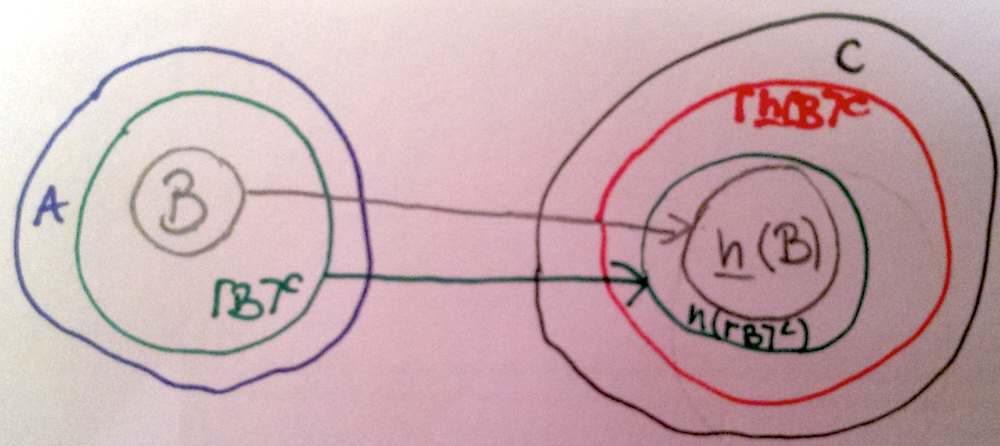
\includegraphics[scale=0.08]{Abbildungen/37}\caption{Abschlüsse und Homomorphismen}
\end{figure}

\subsection{Quotient}

\subsubsection{Kongruenz}

\paragraph{Definition 38 Kongruenzrelation}
Äquirel \&: 
$
x\equiv^{w}x',\, f^{A}(x)=y, f^{A}(x')=y' \, \Rightarrow  \, y\equiv^{v}y'
$

\paragraph{Proposition 39 Schnitt von Kongruenzen}
$\left(\equiv_{i}\right)_{i\in I}$ auf A: $\bigcap_{i\in I}\equiv^{i}$ ist Kongruenz auf A.

\subsubsection{Verband}

\paragraph{Corollary 40 Verband von Kongruenzen}
Die Menge $\mathfrak{C}^{A}=\{\equiv\,::\,\equiv\textrm{ist Kongruenz auf }A\}$
von Kongruenzrelationen auf einem algebraischen System $A$ ist ein vollständiger Verband bis auf Inklusion.

\subsubsection{Abschluss Operator}

\paragraph{Corollary 41 Abschluss Operator}
Kleinste Kongruenz $\left\lceil r\right\rceil _{A}$ auf
$A$ die $r$ enthält.

\subsubsection{Kernel}

\paragraph{Definition 42 Kern eines Homomorphismus}
Kern $h^\equiv$ beinhaltet all die Elemente, die durch den Homomorphismus $h$ auf das Gleiche abgebildet werden.
$h_{s}^{\equiv}=\{(a_{1},a_{2})\,::\, h_{s}(a_{1})=h_{s}(a_{2})\}$

\paragraph{Proposition 43 Kern}
$h^\equiv$ ist eine Kongruenz auf der $h$-Domain.

\paragraph{Proposition 44 Kern einer Komposition}
$m^\equiv \subseteq (n \circ m)^\equiv$ 


\subsubsection{Quotient}

\paragraph{Definition 45 Quotient}
Gegeben System $A$ und $\equiv$ auf A. Der Quotient $A_\equiv$ 
\begin{enumerate}
\item Kongruente Elemente der Trägermenge in eine Äquivalenzklasse schmeissen.
\item $f^{A_{|\equiv}}([x]^{w})=[y]^{v},\,\textrm{wenn }f^{A}(x)=y$
\end{enumerate}

\paragraph{Proposition 46 Quotient von totalen Systemen}
Jeder Quotient eines totalen Systems ist total.

\subsubsection{Natürlicher Homomorphismus}

\paragraph{Proposition 47 Natürlicher Homomorphismus}
Bildet Elemente der Trägermengen in ihre jeweilige Äquivalenzklasse ab ($\equiv : A \rightarrow A_{|\equiv}$). 

\paragraph{Proposition 48 Natürlicher Homomorphismus}
Jeder natürlicher Homomorphismus ist geschlossen.

\paragraph{Proposition 49 Kongruenz Theorem}
$\equiv^{1}$ und $\equiv^{2}$ sind Kongruenzen auf $A$, sodass $\equiv^{1}\,\subseteq\,\equiv^{2}$, dann gibt es einen Homomorphismus $\equiv^{2-1}:A_{|\equiv^{1}}\rightarrow A_{|\equiv^{2}}$
mit $\equiv^{2-1}\circ\equiv^{1}\,=\,\equiv^{2}$.


\subsubsection{Operatoren auf Relationensfamilien}

\paragraph{Proposition 50 Operatoren auf Relationensfamilien}

\begin{enumerate}
\item Symmetrie
\item Reflexivität
\item $r^1_s = r_s$
\item Rekursiver Verkettung 
\item $r^*$ = Vereinigung von 1 bis 4
\item $c^0(r)_s = r_s$
\item $\textrm{c}^{i+1}(r)_{s}=\textrm{c}^{i}(r)_{s}\cup\left\{ \left(y_{i},y'_{i}\right)::f\in O_{w,psq},i=|p|+1,x\left(\textrm{c}^{i}(r)\right)^{w}x',f^{A}(x)=y,f^{A}(x')=y'\right\}$
\item Vereinigung von 6 und 7
\end{enumerate}


\paragraph{Lemma 51}

\begin{enumerate}
\item $r^*$ ist Familie transitiver Relationen.
\item $c^*(r)$ erfüllt Kongruenzbedingungen (Definition 38)
\end{enumerate}


\paragraph{Lemma 52}
Wenn eine Relation $r\subseteq A\times A$ reflexiv ist
und $r\subseteq s\subseteq A\times A$, dann ist $s$ auch reflexiv.


\paragraph{Lemma 53}
Gegeben symmetrische Relation $r$, dann $c^*(r)$ und $r^*$ auch symmetrisch.


\paragraph{Lemma 54}
Gegeben Relation $r$ auf einem totalen $A$. R erfüllt Kongruenzbedingung (Def 38). Dann erfüllt auch $r^*$ die Kongruenzbedingung.


\paragraph{Proposition 55 Konstruktion der generierten Kongruenz}
$A$ total und $r$, dann $\left\lceil r\right\rceil =\left(c^{*}\left(sym\left(r\cup r^{0}\right)\right)\right)^{*}$.

\section{Mono, Epi und Isomorphismen}

\subsection{Isomorphismus}

\paragraph{Definition 57 Sektion, Retraktion und Isomorphismus}
Morphiums $m: A \rightarrow B$ in einer Kategorie $C$.
\begin{enumerate}
\item$m$ ist Sektion wenn $m^{-1} \circ m = id_A$
\item$m$ ist Retraktion  wenn $m \circ m^{-1}  = id_B$
\item $m$ ist Isomorphismus wenn 1 und 2.
\end{enumerate}

\paragraph{Proposition 58/59 Kompositionen von Sektion/Retraktion}
\begin{enumerate}
\item $n, m$ Sektionen/Retraktionen $\Rightarrow$ $n \circ m$ Sektion/Retraktion.
\item $n \circ m$ Sektion/Retraktion $\Rightarrow$ m ist Sektion/ n ist Retraktion.
\end{enumerate}

\paragraph{Proposition 60 Eigenschaften von Isomorphismen}
\begin{enumerate}
\item Alle Identitäten sind Isomorphismen
\item $m$ Isomorphismus $\Rightarrow m^{-1}$ Isomorphismus.
\item $n, m$ Isomorphismen $\Rightarrow n \circ m$ Isomorphismus.
\item $n \circ m$ Isomorphismus und (m Retraktion oder n Sektion) $\Rightarrow $ m und n Isomorphismen.
\item Isomorphismus $i: a \rightarrow b \Rightarrow a \approx b$ ist eine Äquivalenz.
\end{enumerate}

\paragraph{Proposition 61 Isomorphismus in Set}
Kategorie Set, Map $f: a \rightarrow b$
\begin{enumerate}
\item $f$ ist Sektion, wenn $f$ injektiv ist und $a \neq \emptyset$
\item $f$ ist Retraktion, wenn $f$ surjektiv 
\item $f$ ist Isomorphismus, wenn $f$ bijektiv
\end{enumerate}

\paragraph{Proposition 62 Notwendige Bedingungen für Isomorphismen in $Sys(\Sigma)$}
$h: A \rightarrow B$ ist Isomorphismus in $Sys(\Sigma) \Rightarrow$
\begin{enumerate}
\item $h$ ist injektiv in allen Komponenten
\item $h$ ist surjektiv in allen Komponenten
\item $h$ ist voll
\end{enumerate}
 
\paragraph{Proposition 63 Hinreichende Bedingungen für Isomorphismen in $Sys(\Sigma)$}
Wenn $h$ bijektiv (Prop 62: 1 und 2) und voll (Prop 62: 3) ist, dann ist es ein Isomorphismus.

\paragraph{Corollar 64 Ismomorphismus $Sys(\Sigma)$ und $\underline{Sys}(\Sigma)$ }
\begin{enumerate}
\item Die Isomorphismen und $Sys(\Sigma)$ sind bijektive und volle Homomorphismen.
\item Die Isomorphismen und $\underline{Sys}(\Sigma)$ sind bijektive Homomorphismen.
\end{enumerate}

\subsection{Generelle Mono- und Epimorphismen}

\begin{multicols}{2}{}
\columnseprule1pt

\textbf{\underline{Monomorphismus}}

\textbf{Definition 65 (Def)} \\
$m \circ p = m \circ q \Rightarrow p = q$

\textbf{Proposition 66} \\
Jede Sektion ist monisch.

\textbf{Proposition 67 (Komposition)} \\
(1) $n,m$ monic $\Rightarrow n \circ m$ monic. \\
(2) $n \circ m$ monic $\Rightarrow m$ monic.
\\

\textbf{Proposition 68 (Geschlossen unter Iso)} \\
$m: a \rightarrow b$ ist monisch, $a \approx a'$, $b \approx b'$ $\Rightarrow \approx \circ \, m \, \circ \approx: a' \rightarrow b'$ ist mono. 

\textbf{Definition 69 (Abstraktes Subobjekt)} \\
Abstraktes Subobjekt ($a,m:a\rightarrowtail b$) eines Objektes $b$ in Kategorie $C$ \\ - ist ein Objekt $a \in C$ \\ - zusammen mit einem Mono $m:a\rightarrowtail b$

Zwei Subobjekte \\ - $(a_{1},\, m_{1}:a_{1}\rightarrowtail b)$ \\
- $(a_{2},\, m_{2}:a_{2}\rightarrowtail b)$  \\ 
des selben Objektes $b$ sind die selben abstrakten Subobjekte wenn es einen Iso $\approx:a_{1}\rightarrow a_{2}$ gibt, so dass $m_{1}=m_{2}\,\circ\approx$.


\columnbreak
\textbf{\underline{Epimorphismus}}

\textbf{Definition 73 (Def)} \\
$p \circ e = q \circ e \Rightarrow p = q$

\textbf{Proposition 74 } \\
Jede Retraktion ist episch.

\textbf{Proposition 75 (Komposition)} \\
(1) $n,m$ epic $\Rightarrow n \circ m$ epic. \\
(2) $n \circ m$ epic $\Rightarrow n$ epic.\\



\textbf{Proposition 76 (Epi ist abstr. 'notion')} \\
$m: a \rightarrow b$ ist episch, $a \approx a'$, $b \approx b'$ $\Rightarrow \approx \circ \, m \, \circ \approx: a' \rightarrow b'$ ist episch. 

\textbf{Definition 77 (Abstrakter Quotient)} \\
Abstrakter Quotient ($b,e: a \twoheadrightarrow b$)  eines Objektes $a$ in Kategorie $C$ \\ - ist ein Objekt $b \in C$ \\ - zusammen mit einem Epi $e:a \twoheadrightarrow b$

Zwei Quotienten \\ - $(b_{1},\, e_{1}:a \twoheadrightarrow b_1)$ \\
- $(b_{2},\, e_{2}:a \twoheadrightarrow b_2)$  \\ 
des selben Objektes $a$ sind die selben abstrakten Quotienten, wenn es einen Iso $\approx:b_{1}\rightarrow b_{2}$ gibt, so dass $ \approx \circ \, e_{1}=e_{2} $.


\end{multicols}
\newpage

\begin{multicols}{2}
\columnseprule1pt

\textbf{\underline{Monomorphismus}} \\

\textbf{Proposition 70 (Monische Retraktion)} \\
Eine monische Retraktion ist ein Isomorphismus.

\textbf{Proposition 71 (Mono in Set)} \\
Hom. in $Set$ ist monisch $\Leftrightarrow$  er injektiv ist. \\
\\
\\
\\
\\
\\

\textbf{Proposition 72 (Mono in $Sys(\Sigma)$)} \\
Hom. in $Sys(\Sigma)$ ist monisch $\Leftrightarrow$  er injektiv in allen Komponenten ist.
\\
\\

\columnbreak
\textbf{\underline{Epimorphismus}}

\textbf{Proposition 78 (Epische Sektionen)} \\
Eine epische Sektion ist ein Isomorphismus

\textbf{Proposition 79 (Epi in Set)} \\
Hom. in $Set$ ist episch $\Leftrightarrow$ er surjektiv ist.

\textbf{Proposition 80 (Hinreichende Bedingungen für Epis in $Sys(\Sigma)$)} \\
Jeder surjektive Homomorphismus in $Sys(\Sigma)$ ist episch.

\textbf{Proposition 82 (Epi in $Sys(\Sigma))$)} \\
Hom. in $Sys(\Sigma)$ ist episch $\Leftrightarrow$  das kleinste, geschlossene Subsystem von $B$ induziert durch das Bild von $h$ übereinstimmt mit $B$, das heißt: $\left\lceil h(A)\right\rceil ^{C}=B$ .

\end{multicols}

\subsection{Spezielle Mono- und Epimorphismen}

\begin{multicols}{2}{}
\columnseprule1pt

\textbf{\underline{Extremale Monomorphismus}}

\textbf{Definition 83 (Extremaler Mono)} \\
Mono $m: a \rightarrow b$ ist extremal, wenn für jede Zerlegung $m = f \circ e$
gilt: ist $e$ episch dann ist $e$ auch Iso.

\textbf{Proposition 84 } \\
Jede Sektion ist ein extremaler Mono.

\textbf{Proposition 85 (Komposition)} \\
$n \circ m$ extremal Mono $\Rightarrow m$ extremal Mono.


\columnbreak
\textbf{\underline{Extremale Epimorphismus}}

\textbf{Definition 89 (Extremale Epis)} \\
Epi $e: a \rightarrow b$ ist extremal, wenn für jede Zerlegung $e = m \circ f$
gilt: ist $m$ monisch dann muss $m$ auch Iso sein.

\textbf{Proposition 90 } \\
Jede Retraktion ist ein extremaler Epi.

\textbf{Proposition 91 (Komposition)} \\
$e \circ f$ extremal Epi $\Rightarrow e$ extremal Epi.


\end{multicols}

\newpage

%
\begin{multicols}{2}{}
\columnseprule1pt

\textbf{\underline{Extremale Monomorphismus}}

\textbf{Proposition 86 (Extr. Mon. ist abstr. 'Notion') } \\
$m: a \rightarrow b$ ist extremaler Mono, $a' \approx a$, $b \approx b'$ $\Rightarrow \approx \circ \, m \, \circ \approx$ ist extremaler Mono. 
\\
\\
Notiz: Jeder Mono in $Set$ ist extremal.
\\
\\
\\
\\
\textbf{Proposition 87 (Extr. Mono in $Sys(\Sigma)$) } \\
Hom. in $Sys(\Sigma)$ ist extremaler Mono $\Leftrightarrow$  er injektiv und geschlossen.


\columnbreak
\textbf{\underline{Extremale Epimorphismus}}


\textbf{Proposition 92 (Extr. Epi ist abstr. 'Notion') } \\
$e: a \rightarrow b$ ist extremaler Epi, $a' \approx a$, $b \approx b'$ $\Rightarrow \approx \circ \, e \, \circ \approx$ ist extremaler Epi. 
\\
\\
Notiz: Jeder Epi ist $Set$ ist extremal. Extremale Epis sind ein geeignetes Modell zur Abstraktion von Quotienten in $Sys(\Sigma)$

\textbf{Proposition 93 (Extr. Epi in $Sys(\Sigma)$) } \\
Hom. in $Sys(\Sigma)$ ist extremaler Epi  $\Leftrightarrow$  er surjektiv und voll.
\end{multicols}


\subsection{Faktorisierungssysteme}

\subsubsection{Faktorisierungssysteme}

\paragraph{\defi 95 Faktorisierungssystem}
$\mathcal{E}$ und $\mathcal{M}$ sind Klassen von Morphismen in $C$.
$(\mathcal{E}$ und $\mathcal{M})$ ist ein Faktorisierungssystem, wenn
\begin{enumerate}
\item Jeder Morphismus $p$ lässt sich in $p = m \circ e$ zerlegen.
\item $\mathcal{E}$ und $\mathcal{M}$ sind geschlossen unter Komposition mit Isomorphie
\item Wenn $m \circ p \, = \, q \circ e$, dann gibt es einen eindeutigen Morphismus $d$ (Diagonale), so dass $m \circ d = q$ und $d \circ e = p$ (siehe \ref{fig:diagonale}).
\end{enumerate}

\begin{figure}[h]
\label{fig:diagonale}
\noindent \centering{}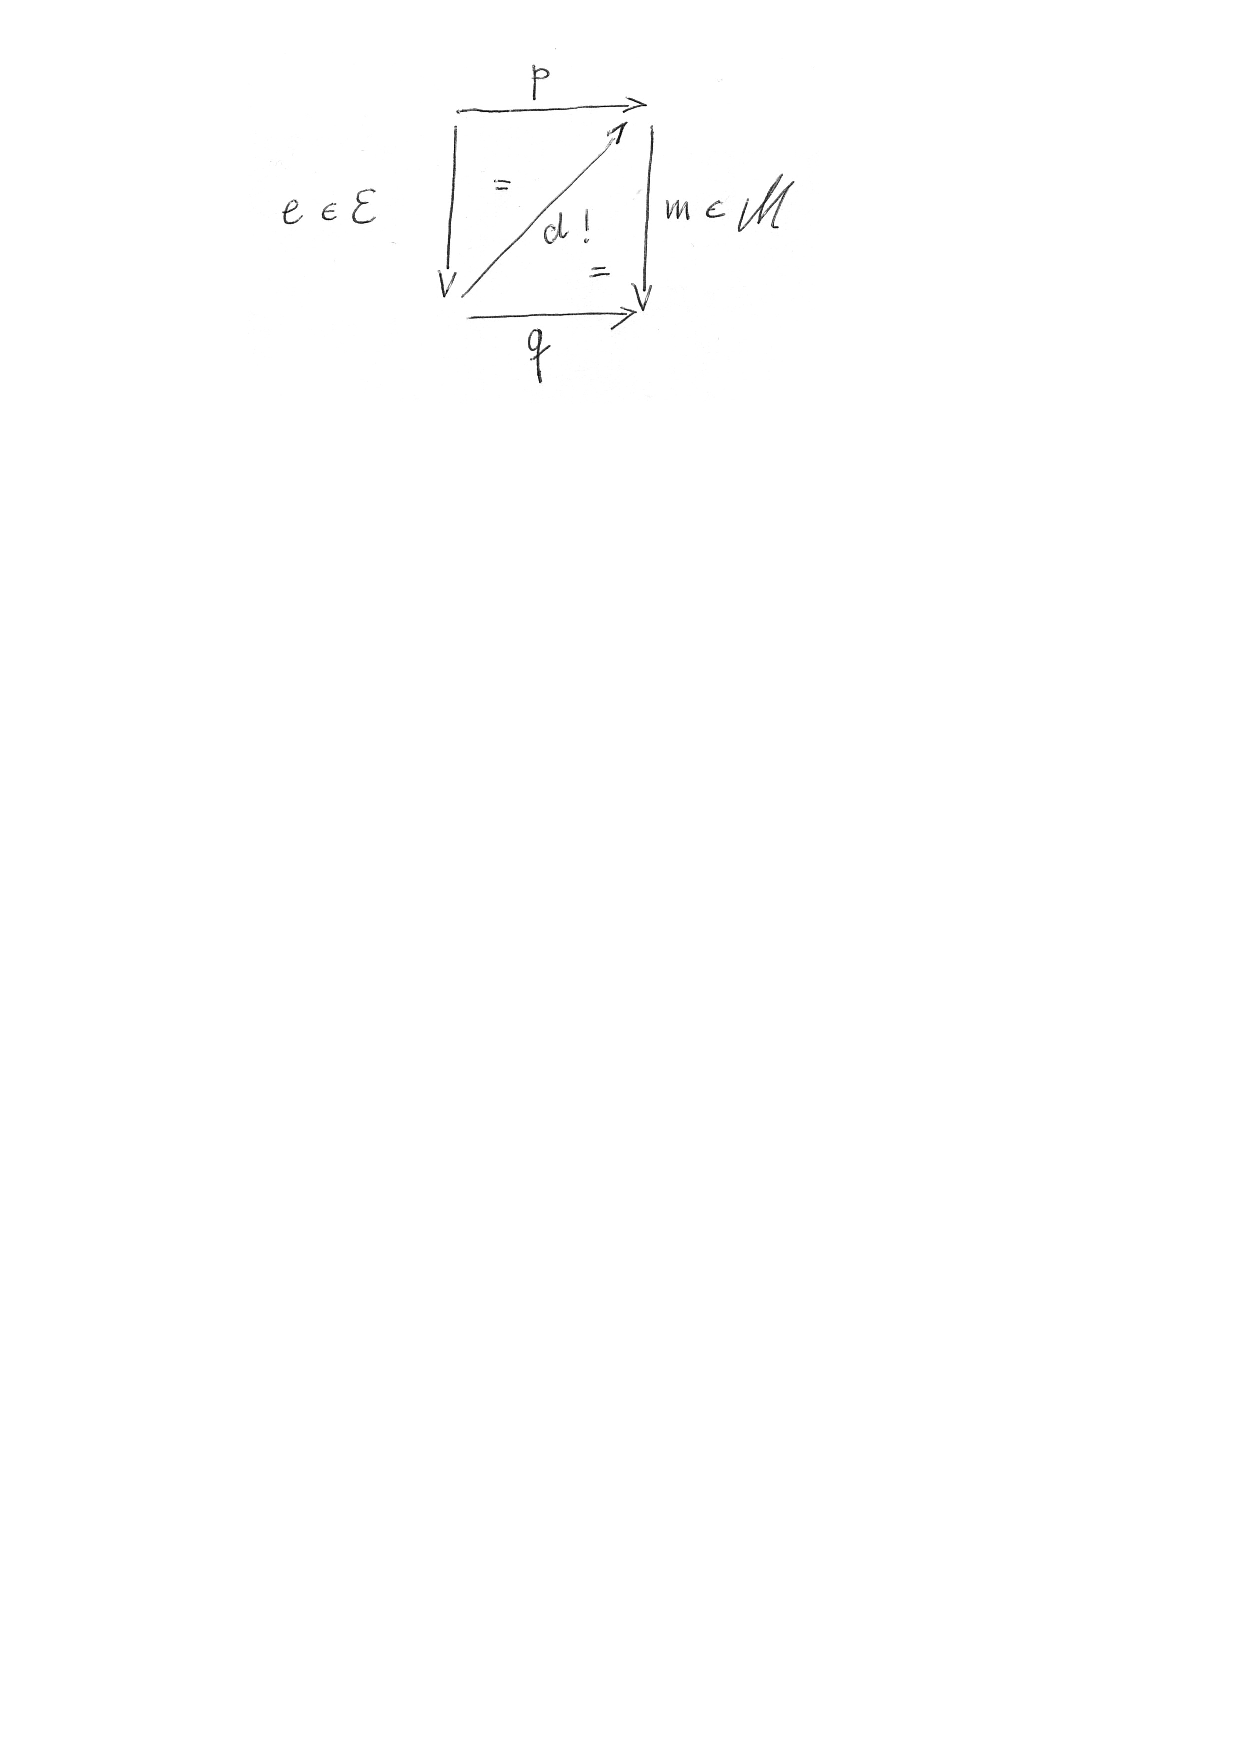
\includegraphics[scale=0.5]{Abbildungen/Diagonal}\caption{Diagonale}
\end{figure}

\paragraph{\prop 96 Eindeutige Faktorisierung}
Faktorisierungen sind eindeutig bis auf Isomorphie:

\begin{enumerate}
\item $(e_{1}:a\rightarrow c_{1},m_{1}:c_{1}\rightarrow b), \\ (e_{2}:a\rightarrow c_{2},m_{2}:c_{2}\rightarrow b)$ sind zwei Faktorisierungen für den selben Morphismus \\ $p:a\rightarrow b$,
\, \, d.h. $m_{1}\circ e_{1}=p=m_{2}\circ e_{2}$ \\
$\Rightarrow$ es gibt Iso $i:c_{1}\rightarrow c_{2}$ mit $i\circ e_{1}=e_{2}$
und $m_{2}\circ i=m_{1}$.
\item $(e:a\rightarrow c,m:c\rightarrow b)$
ist Faktorisierung für $p:a\rightarrow b$ und $i:c\rightarrow d$
ist ein Isomorphismus $\Rightarrow $ $(i\circ e:a\rightarrow d,m\circ i{}^{-1}:d\rightarrow b)$
ist auch Faktorisierung für $p:a\rightarrow b$
\end{enumerate}

\begin{figure}[h]
\label{fig:eindeutig_diagonale}
\noindent \centering{}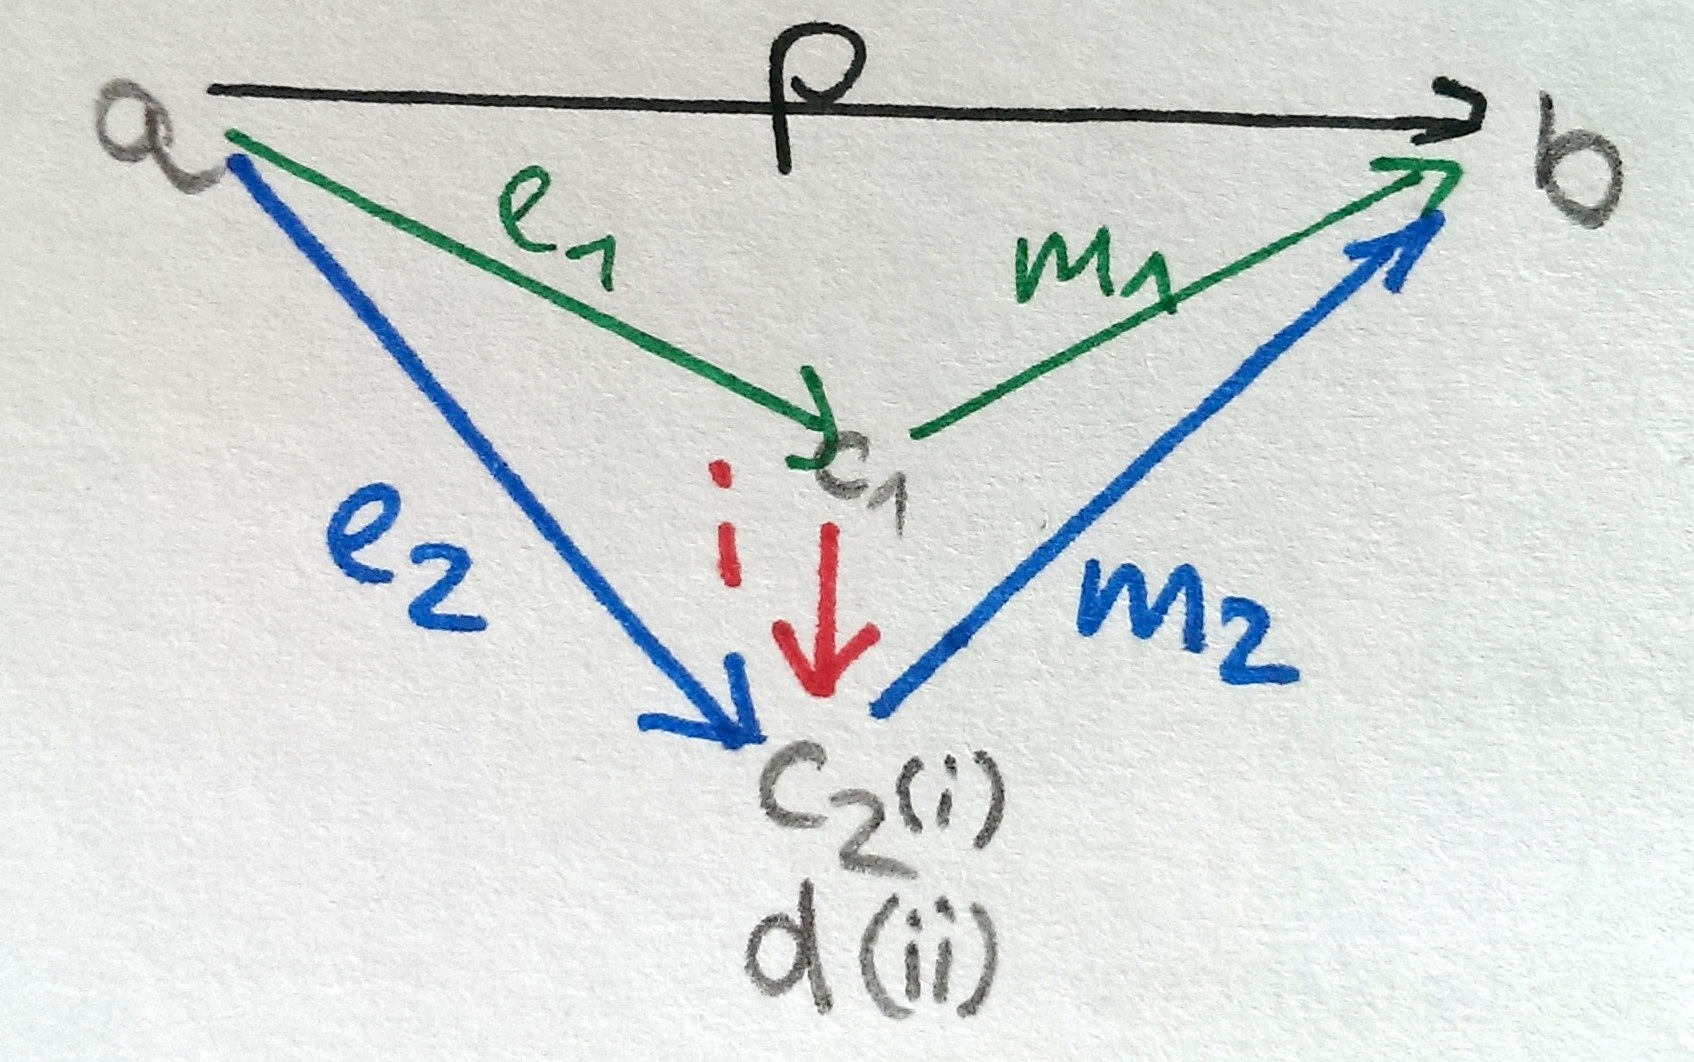
\includegraphics[scale=0.1]{Abbildungen/eindeutig_diagonale}\caption{Eindeutige Diagonale}
\end{figure}

\paragraph{\prop 96 Komposition}
Wenn $(\mathcal{E},\mathcal{M})$ ein Faktorisierungssystem ist, dann sind die Klassen $\mathcal{E}$ und $\mathcal{M}$ geschlossen unter Komposition.

\paragraph{\prop 97 Epi-/Mono-Faktorisierung in Set}
In Set:  $\mathcal{E}$  \epis und $\mathcal{M}$ \monos

\subsubsection{Homomorphismus Theoreme}


\begin{multicols}{2}
\columnseprule1pt

\textbf{\underline{Theorem 1}} 

\textbf{Theorem 99 Homom Theorem 1} \\
$h: A \rightarrow B$ surjektiv und voller Hom. und $k: A \rightarrow C$ ist Hom. so dass $h^\equiv \subseteq k^\equiv$, d.h.
der Kern von $k$ beinhaltet den Kern von $h$ \\ $\Rightarrow$ es gibt einen eindeutigen Homom. \\ $k^*: B \rightarrow C$ so dass $k^* \circ h = k$. \\
$\equiv^h \, \, \, = \, \, \,\equiv^k \, \,\Rightarrow k^*$ ist injektiv.


\columnbreak
\textbf{\underline{Theorem 2}} 

\textbf{Theorem 103 Homom Theorem 2} \\
$h: A \rightarrow B$ injektiver Homom. und \\ $k: C \rightarrow B$ ist Hom. so dass $k(C) \subseteq h(A)$ \\ \\ $\Rightarrow$ es  gibt einen eindeutigen Homom. \\ $k^*: C \rightarrow A$ mit $h\circ k^* = k$ \\
$\left\lceil k(C)\right\rceil ^{c}=h(A)$, then $k^{*} \Rightarrow$ $k^*$ ist epi.

\end{multicols}

\newpage 

\begin{multicols}{2}
\columnseprule1pt

\textbf{\underline{Theorem 1}} \\

\textbf{\lem 100 Invarianter Kern} \\
$m$ injektiver Homom. $\Rightarrow \, \, \equiv^{m \circ h} \, \, = \, \, \equiv^h$ für alle Hom, die mit $m$ komponiert werden können.

\textbf{\coro 101 Extremal epische Faktorisierungen in \syssig} \\
$(\mathcal{E}^{x}, \mathcal{M})$ ist ein Faktorisierungssystem wobei $\mathcal{E}^{x}$ extremaler Epi und $\mathcal{M}$ \mono

\textbf{\coro 102 Komposition extremaler Epis} \\
$e_1 : A \rightarrow B$, $e_2 : B \rightarrow C$ sind zwei extremale Epis in \syssig $\Rightarrow \, e_2 \circ e_1$ ist extremaler Epi.

\columnbreak
\textbf{\underline{Theorem 2}}

\textbf{\lem 104 Invariante Sub-Trägermengen} \\
$e: A \rightarrow B$ epi $\Rightarrow \left\lceil h(B) \right\rceil ^{c} = \left\lceil h\circ e(A)\right\rceil ^{c}$ für alle \homos $h: A \rightarrow C$.

\textbf{\coro 105 Extremal mono Faktorisierungen in \syssig} \\
$(\mathcal{E}, \mathcal{M}^{x})$ ist ein Faktorisierungssystem wobei $\mathcal{E}$ Epi und $\mathcal{M}^{x}$ extremaler \mono

\textbf{\coro 106 Komposition extremaler Monos} \\
$m_1 : A \rightarrow B$, $m_2 : B \rightarrow C$ sind zwei extr. Monos in \syssig $\Rightarrow \, m_2 \circ m_1$ ist extr. Mono.
\end{multicols}

\subsubsection{Surjektive / volle injektive Homomorphismen}

\paragraph{\prop 107 Surjektive und volle injektive Homos}
Konzept der surjektiven und Konzept der vollen inkjektiven Homos ist abstrakt. D.h. Homo $h:A \rightarrow B$ surjektiv/voll und injektiv und $A \approx A'$ und $B \approx B'$ $\Rightarrow \approx \, \, \circ \, \, m \, \, \circ \approx$ ist surjektiv/voll und injektiv.

\paragraph{\coro 109 Surjektive / voll injektive Faktorisierung in \syssig}
($\mathcal{S}$, $\mathcal{FI}$) Faktorisierungssystem in \syssig wobei $\mathcal{S}$ die Klasse aller surjektiven und $\mathcal{FI}$ aller vollen injektiven Morphismen ist.


\end{document}